\documentclass{article}
\usepackage{fancyhdr} % Required for custom headers
\usepackage{lastpage} % Required to determine the last page for the footer
\usepackage{extramarks} % Required for headers and footers
\usepackage{graphicx} % Required to insert images
%\usepackage{lipsum} % Used for inserting dummy 'Lorem ipsum' text into the template
\usepackage{amsmath}
%\usepackage{amsfont}
%\usepackage{amssymb}

\usepackage{multicol}
% Margins
\topmargin=-0.5in
\evensidemargin=0in
\oddsidemargin=-0.5in
\textwidth=7.5in
\textheight=9.0in
\headsep=0.25in 


\pagestyle{fancy}

\rhead{M. Adam} % Top right header
\lhead{Gluten Free Crêpes}
\chead{ }
%\title{}

\begin{document}
%
%PRELIMINARIES:
%
%
%Begin by preheating the oven to 350 $^o$F
%
%\bigskip
%
%\bigskip

\begin{multicols}{2}
Ingredients for the dry mix (which can be stored):
\begin{itemize}
\item 1 cup gluten-free sweet rice flour
\item 1 cup ground hazelnuts
\item 1 cup sweet white sorghum flour (like Bob's Red Mill)
\item 1 cup teff flour (Bob's Red Mill makes this too)
\item 1 \& 1/2 tsp xantham gum (Bob's Red Mill makes this too)
\end{itemize}
\medskip
For the rèpe batter:
\begin{itemize}
\item 3 eggs
\item 1 cup milk
\item 1/3 cup sugar
\item 1 tsp vanilla extract
\item 3/4 cup GF crêpe flour mix (above)
\item Butter for the crêpe pan

\end{itemize}



\columnbreak

Directions:
\begin{enumerate}
\item In a container or a bowl, add the teff flour, sweet white sorghum flour, gluten-free sweet rice flour, ground hazelnuts, and lastly add in the xantham gum.

\item Shake it up if in a container, or mix it well if you did it in a bowl.

\item Preheat your flat crêpe pan to medium to high heat. Crack 3 eggs in a bowl and then add in some milk, sugar, and vanilla extract. Whisk this mixture for a few minutes.

\item Measure out 3/4 cup of your crêpe mixture and add it into the egg mixture. Whisk the batter together and you have your crêpe batter! It will look runny but that is right.

\item Take a little bit of butter and coat the heated pan. Pour approximately 1/3 cup of batter into the center of the crêpe pan and swivel it around with a back and forth shaking motion until you have a thin, round crêpe.

\item Allow crêpe to cook until edges become golden brown, then flip and briefly allow the other side to cook. (10-15 seconds) Slide it right off the pan to a plate.

\item Dress with a small amount of Nutella, jam or maple syrup down the middle, roll up, cut into two pieces and serve warm.
\end{enumerate}




\end{multicols}



\begin{center}
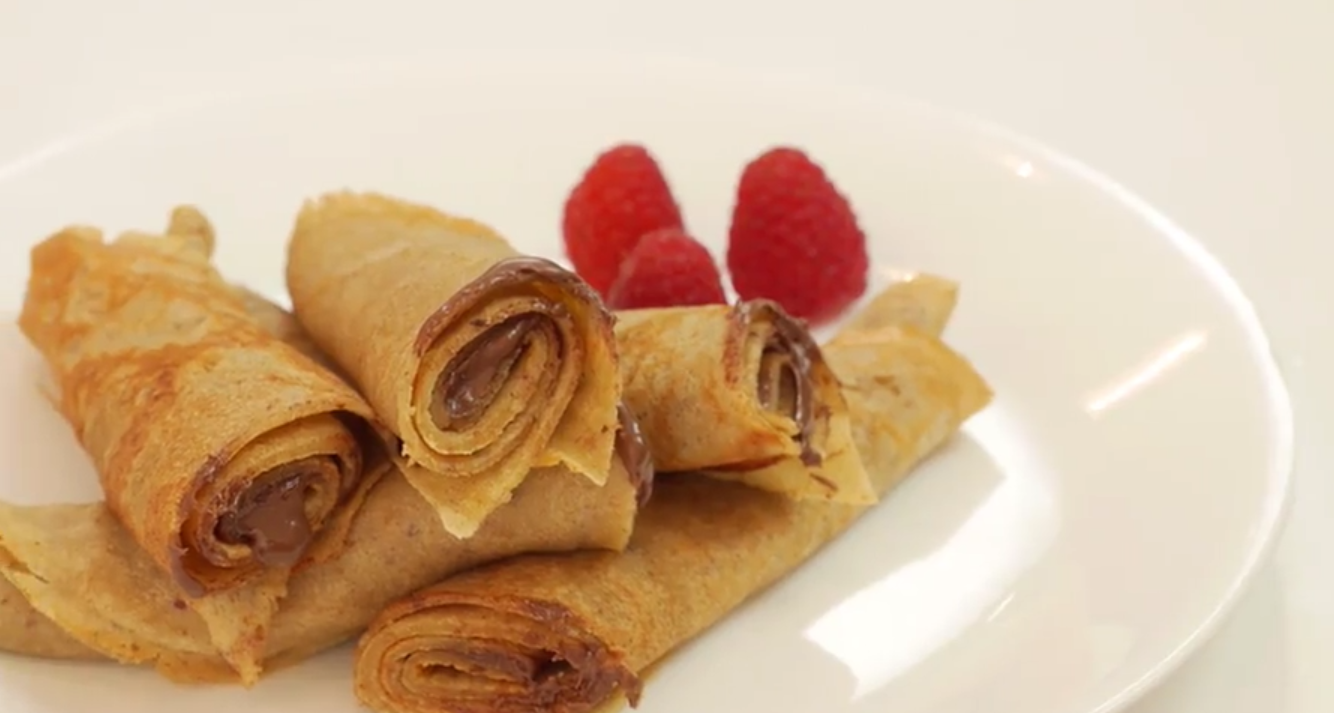
\includegraphics[scale=0.4]{Crepes.png}
\end{center}


\end{document} 











